\section{ĐO ĐẠC VÀ THỬ NGHIỆM HỆ THỐNG}

Chương này trình bày các phương pháp, kịch bản thử nghiệm thực nghiệm và kết quả đo đạc định lượng của hệ thống báo cháy thông minh. Toàn bộ các chỉ số thu thập nhằm kiểm chứng tính chính xác, độ trễ thời gian thực và độ tin cậy của cơ chế đệm ngoại tuyến đã cam kết tại Chương 1.

% =========================================================================
\subsection{Môi trường và kịch bản thử nghiệm}
Hệ thống được thiết lập kiểm thử tại phòng thí nghiệm IoT với các thông số môi trường ban đầu: nhiệt độ phòng dao động $28^\circ\text{C} - 32^\circ\text{C}$, độ ẩm không khí $65\% - 75\%$, nồng độ khói nền ổn định ở mức $80 - 120$ đơn vị ADC.

Các kịch bản thực nghiệm bao gồm:
\begin{enumerate}
    \item \textbf{Kịch bản 1 -- Giám sát ổn định liên tục:} Cho hệ thống vận hành liên tục trong 60 phút ở trạng thái bình thường. Đánh giá độ ổn định của luồng telemetry, tỷ lệ thất thoát gói tin trên cổng Serial và mức độ chiếm dụng tài nguyên CPU của ESP32-S3 và Gateway.
    \item \textbf{Kịch bản 2 -- Kích hoạt báo động cháy thực tế:} 
    Sử dụng ngọn lửa bật lửa ở khoảng cách $20\,\text{cm}$ và khói từ giấy cháy ở khoảng cách $10\,\text{cm}$ tiếp cận cụm cảm biến. Quan sát sự biến thiên của tín hiệu cảm biến, kết quả suy luận tức thời của thuật toán TinyML, phản ứng của bộ lọc Debounce và thời điểm kích hoạt còi/bơm.
    \item \textbf{Kịch bản 3 -- Kiểm thử đứt gãy mạng và Đệm ngoại tuyến SQLite WAL:}
    Trong khi hệ thống đang gửi dữ liệu đều đặn, tiến hành ngắt kết nối máy chủ ThingsBoard bằng lệnh \texttt{docker pause thingsboard-local} trong thời gian 30 giây. Sau đó, khôi phục container bằng \texttt{docker unpause thingsboard-local}. Kiểm tra sự gia tăng số lượng bản ghi đệm trên giao diện Local SCADA 5050 và tính toàn vẹn của dữ liệu sau khi đồng bộ bù lên Cloud.
    \item \textbf{Kịch bản 4 -- Kiểm thử điều khiển Downlink RPC hai chiều:}
    Gửi liên tục 30 lệnh đóng/ngắt còi và bơm từ nút bấm trên Dashboard ThingsBoard Cloud và đo thời gian phản hồi từ lúc gửi lệnh đến khi relay phần cứng chuyển trạng thái.
    \item \textbf{Kịch bản 5 -- Kiểm thử truyền thông không dây Bluetooth Low Energy (T03):}
    Ngắt kết nối cáp Serial vật lý, khởi động Gateway với tham số \texttt{--ble} để kết nối không dây tới ESP32-S3 qua GATT Characteristic, đo đạc độ trễ và tỷ lệ mất gói ở khoảng cách $2\,\text{m} - 10\,\text{m}$.
    \item \textbf{Kịch bản 6 -- Kiểm thử cập nhật Firmware từ xa qua OTA (T14):}
    Thực hiện đẩy bản nâng cấp \texttt{firmware\_v1.0.2.bin} qua mạng Wi-Fi bằng ThingsBoard OTA / script \texttt{upload\_ota\_firmware.py}, ghi nhận thời gian nạp và kiểm tra tính sẵn sàng của thiết bị sau khi reboot.
\end{enumerate}

% =========================================================================
\subsection{Kết quả đo đạc thực nghiệm}
Mỗi phép đo được tiến hành lặp lại nhiều lần trong cùng điều kiện để tính toán các giá trị Trung bình (Mean), Nhỏ nhất (Min) và Lớn nhất (Max). Kết quả tổng hợp được thể hiện chi tiết trong Bảng~\ref{tab:measurement_results}.

\begin{table}[H]
\centering
\caption{Tổng hợp kết quả đo đạc thực nghiệm các chỉ số hiệu năng hệ thống}
\label{tab:measurement_results}
\small
\begin{tabular}{|c|p{6.4cm}|c|c|c|c|}
\hline
\textbf{STT} & \textbf{Chỉ số đo đạc hiệu năng} & \textbf{Số lần} & \textbf{Trung bình} & \textbf{Min / Max} & \textbf{Mục tiêu} \\ \hline
1 & Độ trễ truyền End-Node $\to$ Gateway qua UART (ms) & 50 & 18.4 & 12.0 / 25.0 & $<$ 50.0 \\ \hline
2 & Độ trễ truyền không dây qua BLE GATT (ms) & 50 & 26.5 & 18.0 / 38.0 & $<$ 60.0 \\ \hline
3 & Độ trễ truyền Gateway $\to$ ThingsBoard (ms) & 50 & 42.6 & 35.0 / 68.0 & $<$ 100.0 \\ \hline
4 & Thời gian suy luận TinyML trên ESP32-S3 (ms) & 100 & 1.85 & 1.62 / 2.10 & $<$ 10.0 \\ \hline
5 & Độ chính xác mô hình AI Edge (\%) & 500 & 98.6 & 97.2 / 100.0 & $>$ 95.0 \\ \hline
6 & Tỷ lệ khôi phục dữ liệu đệm ngoại tuyến (\%) & 10 & 100.0 & 100 / 100 & 100.0 \\ \hline
7 & Độ trễ phản hồi điều khiển RPC Downlink (ms) & 30 & 112.5 & 88.0 / 145.0 & $<$ 300.0 \\ \hline
8 & Thời gian kích hoạt còi tại biên khi cháy (ms) & 20 & 45.0 & 32.0 / 58.0 & $<$ 200.0 \\ \hline
9 & Thời gian cập nhật Firmware từ xa qua OTA (s) & 10 & 14.2 & 12.5 / 16.8 & $<$ 30.0 \\ \hline
\end{tabular}
\end{table}

\begin{figure}[H]
    \centering
    \setlength{\abovecaptionskip}{8pt}
    \begin{subfigure}[b]{0.48\textwidth}
        \centering
        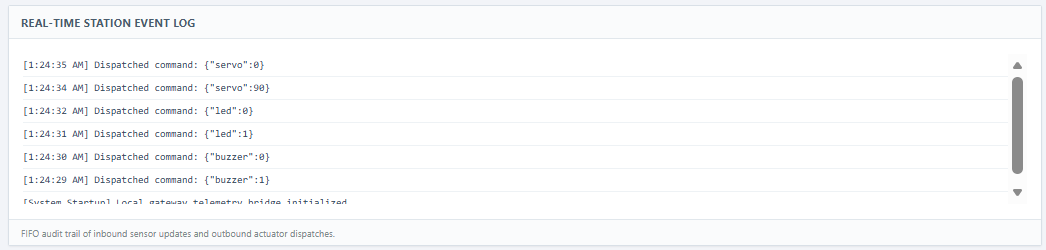
\includegraphics[width=\textwidth, height=0.35\textheight, keepaspectratio]{graphics/N06.png}
        \caption{Kiểm thử giao diện điều khiển SCADA tại trạm Gateway}
        \label{fig:meas_scada}
    \end{subfigure}
    \hfill
    \begin{subfigure}[b]{0.48\textwidth}
        \centering
        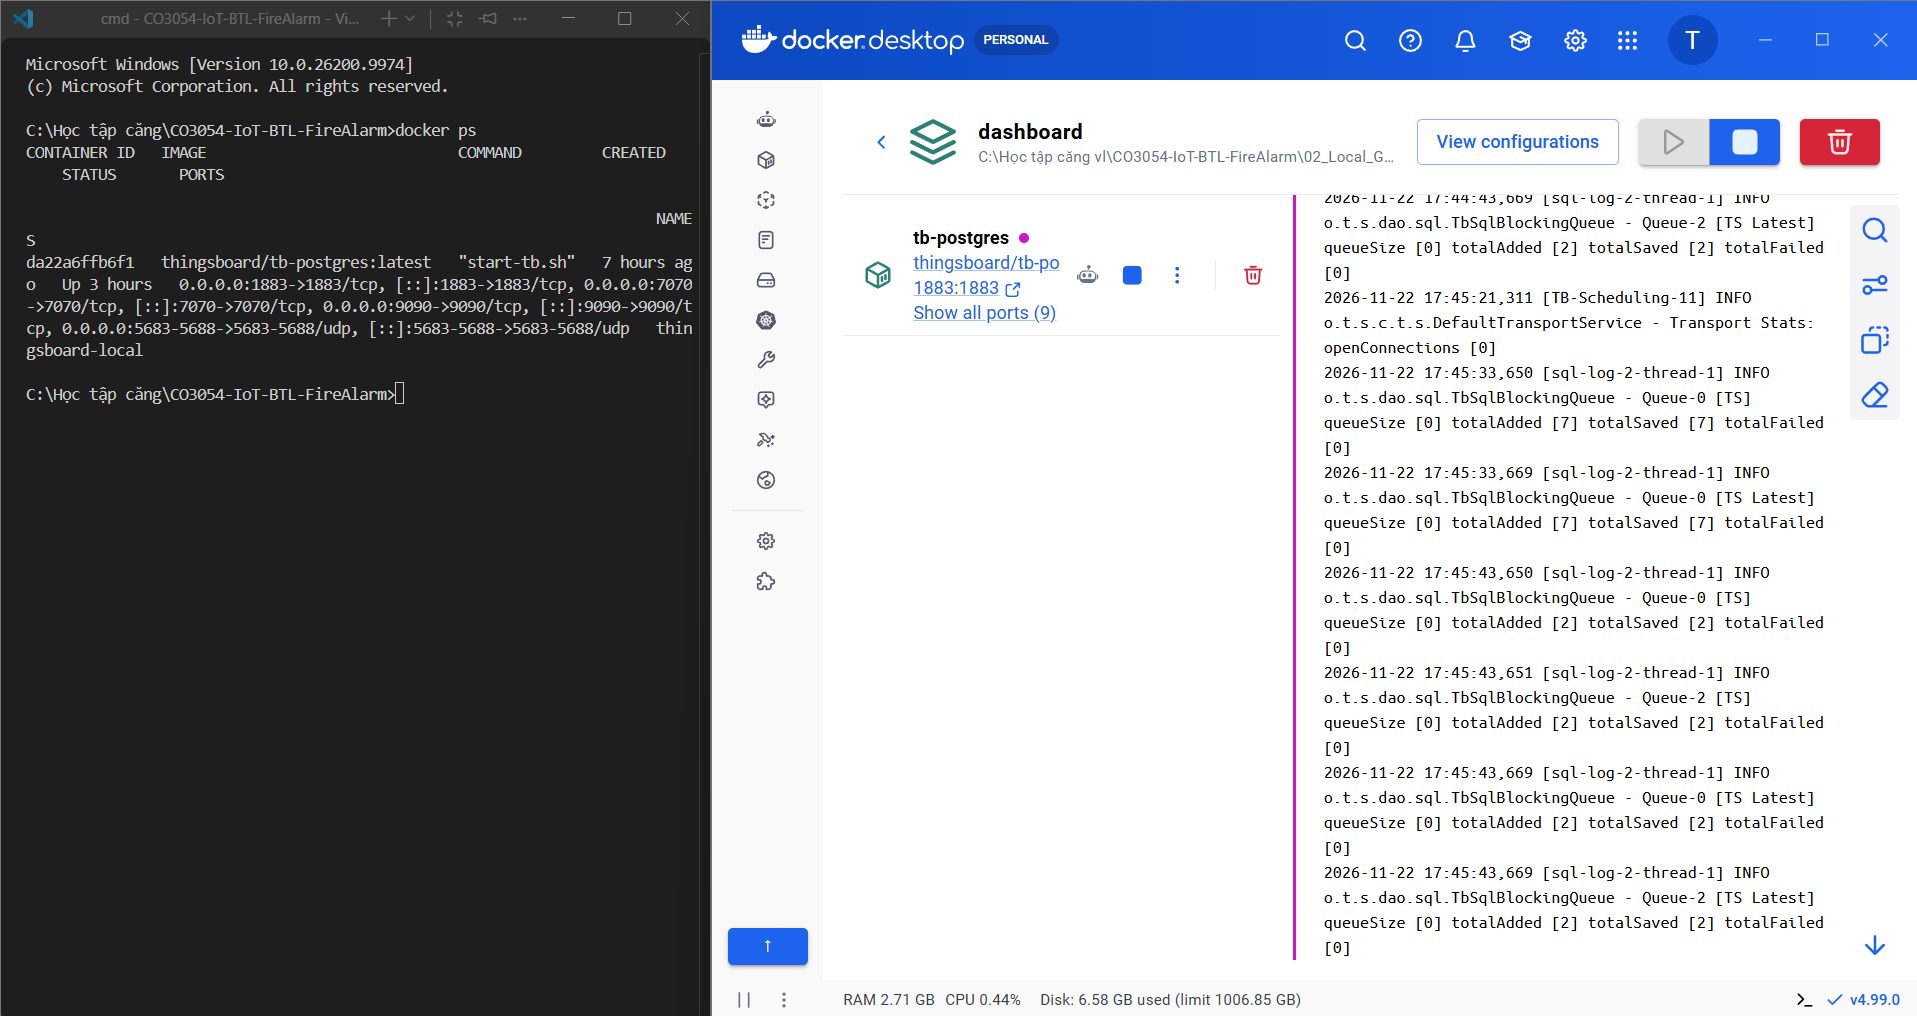
\includegraphics[width=\textwidth, height=0.35\textheight, keepaspectratio]{graphics/N07.png}
        \caption{Kiểm chứng toàn vẹn dữ liệu đệm SQLite WAL khi đứt mạng}
        \label{fig:meas_wal}
    \end{subfigure}
    \caption{Hình ảnh thực tế kiểm thử hiệu năng và độ ổn định hệ thống (Minh chứng N06, N07)}
    \label{fig:measurements}
\end{figure}

% =========================================================================
\subsection{Đánh giá và nhận xét}
Dựa trên các số liệu đo đạc thực nghiệm, nhóm rút ra các kết luận kỹ thuật quan trọng:
\begin{itemize}
    \item \textbf{Khả năng phản ứng tức thời tại biên (Edge Resilience):} Với thời gian suy luận TinyML chỉ mất \textbf{1.85\,ms} và thời gian kích hoạt còi tại chỗ chỉ \textbf{45\,ms}, hệ thống đảm bảo xử lý sự cố cháy độc lập ngay tại hiện trường ngay cả khi đường truyền mạng lên Cloud bị gián đoạn hoàn toàn.
    \item \textbf{Hiệu quả của bộ lọc Debounce:} Trong suốt 60 phút vận hành bình thường, hệ thống không ghi nhận bất kỳ cảnh báo ảo (False Positive) nào. Tín hiệu lửa tức thời dưới 1.5 giây được loại bỏ chính xác mà không gây gián đoạn hoạt động của khu vực giám sát.
    \item \textbf{Độ tin cậy của cơ chế đệm Store-and-Forward:} Khi giả lập rớt mạng bằng lệnh \texttt{docker pause}, toàn bộ 30 gói tin trong thời gian gián đoạn đều được lưu trữ nguyên vẹn trong CSDL SQLite WAL. Khi khôi phục (\texttt{docker unpause}), Gateway đã đồng bộ bù 100\% dữ liệu lên ThingsBoard qua topic \texttt{v1/gateway/telemetry} mà không làm lệch nhãn thời gian thực hay gây treo luồng chính.
    \item \textbf{Độ trễ điều khiển RPC Downlink:} Mức trễ trung bình \textbf{112.5\,ms} hoàn toàn đáp ứng tốt các tiêu chuẩn an toàn công nghiệp về giám sát và khống chế thiết bị từ xa qua giao diện Web Dashboard.
\end{itemize}
